\section{Language and compiler design}

CTFE First apporach was created during implementation of the first compiler for the C-=-1 language\cite{grabski2022compilation}.
The need for a new approach to compiler construction arose due to the unusal characteristics of the language, further described in chapter \ref{language-design}.
Chapter \ref{compiler-design} describes the CTFE First approach and how the compiler is structured. 

\subsection{Design of C-=-1}
\label{language-design}

C-=-1 was designed as a compiled, low-level, non-garbage-collected programming language, similar to C, C++ or Rust.
What diffirentiates C-=-1 are its two founding principles: all code is executable at compile-time and support rich metaprogramming.
The primary purpose of the language was to research how these ideas influence software written in it \cite{grabski2022compilation}.

\subsubsection{Type system}

\subsubsection{Attributes and metaprogramming}

\subsection{Design of the compiler}
\label{compiler-design}

CTFE First compiler has four major components: Frontend, Interpreter, Compiler Interface and Backend.
Figure \ref{CTFE-first-compiler-structure} contains a diagram with an overview of how these pieces interact with eachother, during the compilaton process.
Frontend, described in chapter \ref{frontend}, parses the code in the compiled language and constructs its intermidaite representation, using interpreter's data structures.
It is used to analyze both user code and the Compiler Interface.
After the intermidiate representation is constructed, it is passed on to the Interpreter, which was described in chapter \ref{interpreter}.
Compiler Interface intermidiate representation is then executed, using the user program as data. 
This step converts the semantic model of the program into the backends intermidiate language.
This process has been further explained in chapter \ref{compiler-interface}.
Finaly the Backend generates the executable file.

\begin{figure}
	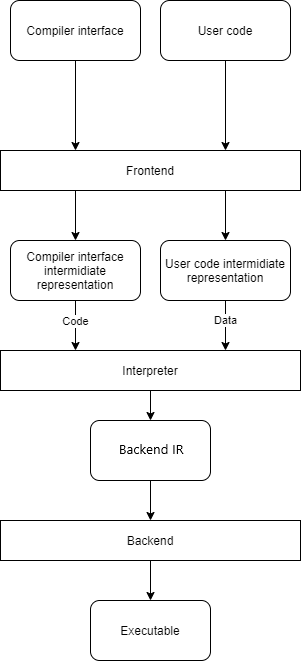
\includegraphics[height=10cm]{pictures/compiler-structure.png}
	\caption{CTFE First compiler structure}
	\label{CTFE-first-compiler-structure}
\end{figure}

\subsubsection{Frontend}
\label{frontend}

\subsubsection{Interpreter}
\label{interpreter}

\subsubsection{Compiler interface} 
\label{compiler-interface}

\subsubsection{Backend}
\label{backend}
